\chapter{Reatores contínuos e processos industriais}\label{ch:b2:continuous-reactors}

No laboratório, uma reação é conduzida em um balão: os reagentes entram, a
mistura é agitada por uma hora, a reação é interrompida e o produto,
isolado. Uma indústria que fabrica o mesmo produto aos milhares de toneladas
trabalha de outra forma. Seu reator nunca se esvazia: os reagentes entram
por uma extremidade, os produtos saem pela outra, dia e noite, e a
composição no interior não muda com o tempo. Duas perguntas substituem
então o ``quanto tempo?'': que tamanho deve ter o reator para uma dada
\omterm{def:b2:continuous-reactors:conversion}{conversão}, e como retirar o calor da reação antes que ele aqueça o reator
até a perda de controle? Este capítulo escreve os balanços de matéria e de
energia dos dois \omterm{def:b2:continuous-reactors:reactors}{reatores contínuos} ideais, o tanque agitado e o tubo,
compara-os e mostra como um reator pode ter vários estados possíveis, um
dos quais é um disparo.

\begin{recall}
O volume do 1.º ano: velocidade de reação, leis de velocidade e ordens,
leis integradas de um reator fechado (agora chamado \omterm{def:b2:continuous-reactors:reactors}{reator em batelada}),
meia-vida, a lei de Arrhenius $k = A\,\mathrm e^{-E_a/RT}$, reações
consecutivas. \Cref{ch:b2:reaction-enthalpy}: calor liberado a pressão
constante; \cref{ch:b2:equilibrium-shifts}: \omterm{def:b2:equilibrium-shifts:single-pass}{conversão por passagem}, \omterm{def:b2:equilibrium-shifts:single-pass}{reciclo}.
Da física: o balanço de um sistema aberto em escoamento estacionário (o que
entra menos o que sai é igual ao que se acumula).
\end{recall}

\begin{omfigure}
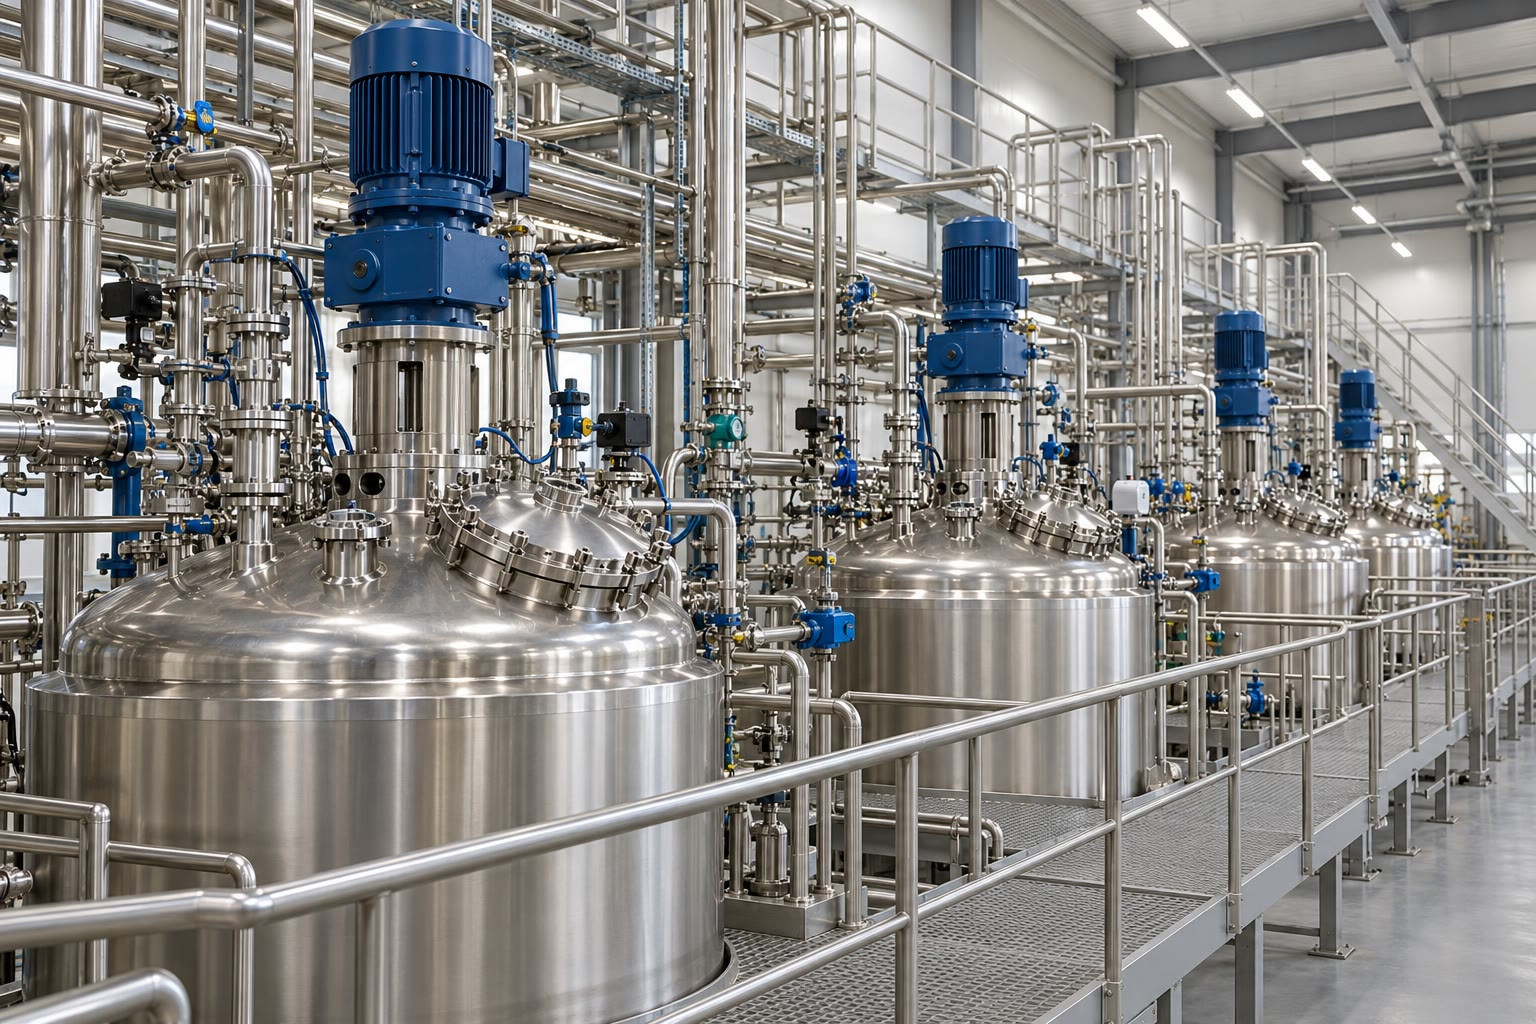
\includegraphics[width=0.6\linewidth]{images/book3/ai/b2-05-stirred-tanks.jpg}

{\small Reatores de tanque agitado em uma indústria química: cada vaso
leva seu motor e seu redutor, e o eixo do agitador desce até a mistura
reacional; as tubulações trazem as alimentações e levam o produto e a água
de resfriamento.}
\end{omfigure}

\section{Da batelada ao contínuo}

\begin{definition}[Tipos de reator]\label{def:b2:continuous-reactors:reactors}
Um \emph{reator em batelada}\index{reator em batelada} é um vaso fechado no qual a
reação ocorre sem entrada nem saída de matéria. Um
\emph{reator contínuo}\index{reator continuo@reator contínuo} é atravessado por um
escoamento estacionário de matéria. Dois reatores contínuos ideais servem
de modelo:
\begin{itemize}
  \item o \emph{reator contínuo de tanque agitado}\index{reator continuo de tanque agitado@reator contínuo de tanque agitado}
(CSTR), tão bem agitado que seu conteúdo é
        uniforme e, portanto, idêntico à corrente que sai dele;
  \item o \emph{reator de escoamento pistonado}\index{reator de escoamento pistonado} (PFR), um tubo
        atravessado pelo fluido sem mistura ao longo do escoamento, cada fatia
        de fluido avançando como um pistão enquanto reage.
\end{itemize}
\end{definition}

Diz-se que um \omterm{def:b2:continuous-reactors:reactors}{reator contínuo} funciona em \emph{regime estacionário} quando
nada muda com o tempo em seu interior: as vazões, as temperaturas e as
composições em cada ponto são constantes. Consideramos uma única reação
$\mathrm A \to$ produtos, uma alimentação líquida de massa específica
constante (de modo que a vazão volumétrica $Q_v$ é a mesma na entrada e na
saída), com concentração $c_{A,0}$ na entrada.

\begin{definition}[Tempo de residência]\label{def:b2:continuous-reactors:residence-time}
O \emph{tempo de residência}\index{tempo de residencia@tempo de residência} de um \omterm{def:b2:continuous-reactors:reactors}{reator contínuo} de
volume $V$ alimentado com a vazão volumétrica $Q_v$ é $\tau = V/Q_v$: o tempo
médio que um volume de fluido passa em seu interior.
\end{definition}

\begin{definition}[Conversão]\label{def:b2:continuous-reactors:conversion}
A \emph{conversão}\index{conversao@conversão} do reagente A é $X = (F_{A,0} -
F_A)/F_{A,0}$, em que $F_{A,0}$ e $F_A$ são as vazões molares de A que
entram no reator e saem dele; para um \omterm{def:b2:continuous-reactors:reactors}{reator em batelada}, $X = (n_{A,0} -
n_A)/n_{A,0}$. A massa específica constante, $X = 1 - c_A/c_{A,0}$.
\end{definition}

A \omterm{def:b2:continuous-reactors:conversion}{conversão} se refere a um reagente e a um reator ou a uma passagem; a
taxa de avanço final do volume do 1.º ano se refere a uma reação e a seu
reagente limitante. Para uma única reação cujo reagente limitante é A, as
duas coincidem.

\begin{proposition}[Reator em batelada]\label{prop:b2:continuous-reactors:batch}
Em um \omterm{def:b2:continuous-reactors:reactors}{reator em batelada} de volume constante, uma reação de primeira ordem
atinge a \omterm{def:b2:continuous-reactors:conversion}{conversão} $X = 1 - \mathrm e^{-kt}$ após o tempo $t$, e uma reação
de segunda ordem com concentrações iniciais iguais $c_0$, a \omterm{def:b2:continuous-reactors:conversion}{conversão} $X =
kc_0t/(1 + kc_0t)$.
\end{proposition}

\begin{proof}
São as leis de velocidade integradas do volume do 1.º ano, $c_A = c_{A,0}
\mathrm e^{-kt}$ e $1/c_A = 1/c_{A,0} + kt$, escritas com $X = 1 -
c_A/c_{A,0}$.
\end{proof}

\section{O reator contínuo de tanque agitado}

\begin{omfigure}
\begin{tikzpicture}[font=\small, >={Stealth}]
  % batch
  \pic[transform shape] at (0,0) {rbflask={0.6}{omDef!20}};
  \node[below] at (0,-0.15) {batelada};
  % CSTR
  \begin{scope}[xshift=4.2cm]
    \draw[thick, fill=omDef!15] (-1.2,0) rectangle (1.2,2.4);
    \draw[thick] (0,3.0) -- (0,0.5);
    \draw[thick, fill=gray!40] (-0.5,0.45) rectangle (0.5,0.6);
    \draw[thick, fill=gray!30] (-0.25,3.0) rectangle (0.25,3.35);
    \draw[->, thick, omDef] (-2.8,2.0) -- (-1.2,2.0) node[pos=0.0, above, anchor=south west, inner sep=1pt] {$Q_v$, $c_{A,0}$};
    \draw[->, thick, omThm] (1.2,0.3) -- (2.5,0.3) node[pos=1, below] {$Q_v$, $c_A$};
    \node[fill=omDef!15, inner sep=1pt] at (0.62,1.5) {$V$, $c_A$};
    \node[below] at (0,-0.15) {tanque agitado};
  \end{scope}
  % PFR
  \begin{scope}[xshift=8.4cm, yshift=1.0cm]
    \draw[thick, fill=omDef!10] (0,0) rectangle (4.2,0.7);
    \fill[omThm!25] (2.0,0) rectangle (2.35,0.7);
    \draw[thick] (2.0,0) -- (2.0,0.7) (2.35,0) -- (2.35,0.7);
    \node[above] at (2.17,0.75) {$\dd V$};
    \draw[->, thick, omDef] (-0.9,0.35) -- (0,0.35) node[pos=0, above] {$F_{A,0}$};
    \draw[->, thick, omThm] (4.2,0.35) -- (5.0,0.35) node[pos=1, above] {$F_A$};
    \node[below] at (1.0,0) {$F_A(V)$};
    \node[below] at (2.1,-1.15) {tubo pistonado};
  \end{scope}
\end{tikzpicture}

{\small Os três reatores ideais. Um balão em batelada; um tanque agitado cujo
conteúdo uniforme é o da corrente de saída; um tubo atravessado em
escoamento pistonado, no qual a vazão de A diminui de fatia em fatia.}
\end{omfigure}

\begin{proposition}[Balanço de um tanque agitado]\label{prop:b2:continuous-reactors:cstr-balance}
Em regime estacionário, um tanque agitado de volume $V$ no qual A desaparece
com a velocidade $r$ (mol por litro e por segundo) satisfaz
\[
  F_{A,0} - F_A - rV = 0, \qquad\text{isto é,}\qquad c_{A,0} - c_A = r\,\tau ,
\]
sendo a velocidade avaliada na composição e na temperatura de saída.
\end{proposition}

\begin{proof}
Balanço de A no tanque durante $\dd t$: o que entra, $F_{A,0}\dd t$,
menos o que sai, $F_A\dd t$, menos o que reage, $rV\dd t$, é igual ao
acúmulo, nulo em regime estacionário. Sendo o tanque uniforme, a velocidade
é a mesma em toda parte e igual à da corrente de saída. Divida por $Q_v$.
\end{proof}

\begin{theorem}[Conversão em um tanque agitado]\label{thm:b2:continuous-reactors:cstr}
Para uma reação de primeira ordem, $X = \dfrac{k\tau}{1 + k\tau}$; para uma
reação de segunda ordem com concentrações de alimentação iguais $c_0$ dos dois
reagentes, $X$ é a raiz em $[0, 1]$ de $Da\,(1 - X)^2 = X$, com $Da =
kc_0\tau$.
\end{theorem}

\begin{proof}
Ordem 1: $r = kc_A$, logo $c_{A,0} - c_A = k\tau c_A$, $c_A = c_{A,0}/(1 + k\tau)$
e $X = 1 - 1/(1 + k\tau)$. Ordem 2: $r = kc_A^2$ (as duas concentrações
continuam iguais), $c_0X = k\tau c_0^2(1 - X)^2$.
\end{proof}

O grupo adimensional $Da = k\tau$ (ou $kc_0\tau$), o número de
Damköhler, compara o \omterm{def:b2:continuous-reactors:residence-time}{tempo de residência} com a escala de tempo da reação:
só ele fixa a \omterm{def:b2:continuous-reactors:conversion}{conversão}.

\begin{method}[Dimensionar um reator]\label{met:b2:continuous-reactors:size-reactor}
\begin{enumerate}
  \item Escreva a lei de velocidade e a \omterm{def:b2:continuous-reactors:conversion}{conversão} $X$ exigida.
  \item A partir do balanço do reator escolhido, encontre o número de
        Damköhler que dá $X$.
  \item Deduza $\tau$ a partir de $Da$ e da constante de velocidade na
        temperatura de trabalho, e $V = \tau Q_v$ a partir da vazão a tratar.
\end{enumerate}
\end{method}

\section{O reator de escoamento pistonado}

\begin{theorem}[Conversão em um reator de escoamento pistonado]\label{thm:b2:continuous-reactors:pfr}
Em regime estacionário, a vazão de A ao longo de um tubo pistonado obedece a
$\dd F_A/\dd V = -r$. Para uma reação de primeira ordem, isso dá $X = 1 -
\mathrm e^{-k\tau}$ e, para uma reação de segunda ordem com alimentações
iguais, $X =
Da/(1 + Da)$: as leis do \omterm{def:b2:continuous-reactors:reactors}{reator em batelada}, com o \omterm{def:b2:continuous-reactors:residence-time}{tempo de residência} no
lugar do tempo.
\end{theorem}

\begin{proof}
Balanço de A na fatia entre $V$ e $V + \dd V$: $F_A(V) - F_A(V + \dd V)
- r\,\dd V = 0$, donde a equação diferencial. Com $F_A = Q_vc_A$ e
$\dd V = Q_v\,\dd t'$ (o tempo $t'$ que uma fatia passou no tubo), ela se escreve
$\dd c_A/\dd t' = -r$: cada fatia é um pequeno \omterm{def:b2:continuous-reactors:reactors}{reator em batelada} que fica
no tubo durante $\tau$. Separando as variáveis para $r = kc_A$, obtém-se $c_A = c_{A,0}
\mathrm e^{-k\tau}$ na saída; para $r = kc_A^2$, $1/c_A - 1/c_0 = k\tau$.
\end{proof}

\begin{omfigure}
\begin{tikzpicture}
\begin{axis}[
  width=0.75\linewidth, height=6cm, xmin=0, xmax=10, ymin=0, ymax=1.05,
  axis x line=bottom, axis y line=left, xlabel={número de Damköhler $k\tau$},
  ylabel={conversão $X$}, tick label style={font=\small},
  label style={font=\small}, clip=false,
  legend style={font=\scriptsize, draw=none, at={(0.98,0.05)}, anchor=south east}]
\addplot[omThm, very thick] table[x=Da, y=pfr] {figdata/out/bachelor-2-reactors-a.dat};
\addplot[omProp, thick] table[x=Da, y=five] {figdata/out/bachelor-2-reactors-a.dat};
\addplot[omProp, thick, dashed] table[x=Da, y=two] {figdata/out/bachelor-2-reactors-a.dat};
\addplot[omDef, very thick] table[x=Da, y=cstr] {figdata/out/bachelor-2-reactors-a.dat};
\legend{escoamento pistonado, 5 tanques em série, 2 tanques em série, 1 tanque agitado}
\draw[dotted] (axis cs:2.303,0) -- (axis cs:2.303,0.9) -- (axis cs:9,0.9);
\fill[omThm] (axis cs:2.303,0.9) circle (1.4pt);
\fill[omDef] (axis cs:9,0.9) circle (1.4pt);
\end{axis}
\end{tikzpicture}

{\small \omterm{def:b2:continuous-reactors:conversion}{Conversão} de uma reação de primeira ordem em função de $k\tau$ nos
reatores ideais. Para 90\,\% de \omterm{def:b2:continuous-reactors:conversion}{conversão}, um tubo pistonado precisa de
$k\tau = \ln 10 = 2.3$; um único tanque agitado, de $k\tau = 9$: quatro
vezes o volume. Tanques em série se aproximam do tubo.}
% (model curves, computed in figdata/bachelor-2/reactors.py)
\end{omfigure}

\begin{proposition}[Tanque ou tubo]\label{prop:b2:continuous-reactors:compare}
Para toda velocidade que aumenta com a concentração de A (toda ordem
positiva), um \omterm{def:b2:continuous-reactors:reactors}{reator de escoamento pistonado} atinge uma dada \omterm{def:b2:continuous-reactors:conversion}{conversão} com
um volume menor que um tanque agitado.
\end{proposition}

\begin{proof}
Pelos balanços, $\tau_{\text{CSTR}} = c_{A,0}X/r(X)$ (a velocidade na
composição de saída) e $\tau_{\text{PFR}} = c_{A,0}\int_0^X\dd X'/r(X')$. Como $r$
diminui quando $X$ aumenta, $1/r(X') \leq 1/r(X)$ em $[0, X]$, logo a
integral é no máximo $X/r(X)$. Graficamente, em um gráfico de $1/r$ em função
de $X$, o $\tau$ do tubo é a área sob a curva e o do tanque, o retângulo de
altura $1/r(X)$ (figura abaixo). Para a ordem 1: $\ln(1 + k\tau) \leq k\tau$,
o mesmo enunciado sob outra forma.
\end{proof}

O tanque agitado trabalha inteiramente na concentração de saída, a mais
baixa do sistema, e portanto na velocidade mais baixa; o tubo aproveita as
concentrações altas perto de sua entrada. As vantagens do tanque estão em
outro lugar: uma temperatura uniforme e fácil de controlar, e uma operação
simples.

\begin{omfigure}
\begin{tikzpicture}
\begin{axis}[
  width=0.62\linewidth, height=5.6cm, xmin=0, xmax=1, ymin=0, ymax=22,
  axis x line=bottom, axis y line=left, xlabel={conversão $X$},
  ylabel={$1/r$ (unidades do modelo)}, tick label style={font=\small},
  label style={font=\small}, clip=false]
\fill[omDef!15] (axis cs:0,0) rectangle (axis cs:0.9,10);
\addplot[omThm, fill=omThm!20, draw=none, domain=0:0.9, samples=60] {1/(1-x)} \closedcycle;
\addplot[black, very thick] table[x=X, y=invr] {figdata/out/bachelor-2-reactors-c.dat};
\draw[omDef, thick] (axis cs:0,10) -- (axis cs:0.9,10) -- (axis cs:0.9,0);
\node[omDef, font=\scriptsize, anchor=south] at (axis cs:0.45,10.2) {tanque agitado: retângulo, $\tau = 9$};
\node[omThm, font=\scriptsize, anchor=west] (pf) at (axis cs:0.05,6.5) {pistonado: área sombreada, $\tau = \ln 10$};
\draw[omThm, ->] (axis cs:0.25,6.0) -- (axis cs:0.3,0.8);
\end{axis}
\end{tikzpicture}

{\small Gráfico de Levenspiel de uma reação de primeira ordem ($k = 1$, $c_{A,0} = 1$).
Para 90\,\% de \omterm{def:b2:continuous-reactors:conversion}{conversão}, o tanque agitado precisa do retângulo inteiro; o
escoamento pistonado, só da área sombreada sob a curva.}
% (model, computed in figdata/bachelor-2/reactors.py)
\end{omfigure}

\begin{proposition}[Tanques em série]\label{prop:b2:continuous-reactors:cascade}
$N$ tanques agitados iguais em série, de \omterm{def:b2:continuous-reactors:residence-time}{tempo de residência} total $\tau$,
convertem uma reação de primeira ordem até $X_N = 1 - (1 + k\tau/N)^{-N}$,
que aumenta com $N$ e tende ao valor do escoamento pistonado, $1 - \mathrm e^{-k\tau}$.
\end{proposition}

\begin{proof}
Cada tanque divide a concentração por $1 + k\tau/N$. E $(1 +
k\tau/N)^{-N} = \exp[-N\ln(1 + k\tau/N)] \to \mathrm e^{-k\tau}$, pois
$N\ln(1 + u/N) \to u$.
\end{proof}

\begin{definition}[Seletividade]\label{def:b2:continuous-reactors:selectivity}
Quando um reagente pode dar vários produtos, a \emph{seletividade}\index{seletividade}
para o produto desejado B é a quantidade de B formada dividida pela
quantidade de reagente consumida (vezes a razão estequiométrica): ela diz
quanto do que reagiu seguiu o caminho certo.
\end{definition}

\begin{proposition}[Um intermediário em um tanque e em um tubo]\label{prop:b2:continuous-reactors:consecutive}
Para reações consecutivas de primeira ordem $\mathrm A \xrightarrow{k_1} \mathrm B
\xrightarrow{k_2} \mathrm C$, com uma alimentação só de A, a concentração
de B na saída é máxima para $\tau = \ln(k_2/k_1)/(k_2 - k_1)$ em um
\omterm{def:b2:continuous-reactors:reactors}{reator de escoamento pistonado} e para $\tau = 1/\sqrt{k_1k_2}$ em um tanque
agitado; o máximo é mais alto no tubo.
\end{proposition}

\begin{proof}
Tubo: as leis da batelada do volume do 1.º ano, $c_B = c_{A,0}\frac{k_1}{k_2 - k_1}
(\mathrm e^{-k_1\tau} - \mathrm e^{-k_2\tau})$, máxima onde a derivada
se anula, $k_1\mathrm e^{-k_1\tau} = k_2\mathrm e^{-k_2\tau}$. Tanque: $c_A =
c_{A,0}/(1 + k_1\tau)$ e o balanço de B, $c_B = k_1\tau c_A - k_2\tau c_B$,
dá $c_B = c_{A,0}k_1\tau/[(1 + k_1\tau)(1 + k_2\tau)]$, cuja derivada
se anula quando $k_1k_2\tau^2 = 1$. A comparação dos máximos é o
\cref{exo:b2:continuous-reactors:10}.
\end{proof}

\section{Balanço térmico e segurança}

\begin{definition}[Elevação adiabática de temperatura]\label{def:b2:continuous-reactors:adiabatic-rise}
A \emph{elevação adiabática de temperatura}\index{elevacao adiabatica de temperatura@elevação adiabática de temperatura}
$\Delta T_{\text{ad}}$ de uma mistura reacional é a elevação de temperatura
que ela sofreria se a reação fosse completa e nenhum calor fosse retirado.
\end{definition}

\begin{proposition}[Elevação adiabática de uma mistura líquida]\label{prop:b2:continuous-reactors:adiabatic}
Para uma mistura de massa específica $\rho$ e capacidade calorífica mássica
$c_p$, na qual o reagente A, à concentração $c_{A,0}$, reage com a entalpia
$\Delta_r H$ por mol de A, a elevação de temperatura na \omterm{def:b2:continuous-reactors:conversion}{conversão} $X$ sem
perda de calor é
\[
  \Delta T = \frac{(-\Delta_r H)\,c_{A,0}\,X}{\rho\,c_p}, \qquad
  \Delta T_{\text{ad}} = \frac{(-\Delta_r H)\,c_{A,0}}{\rho\,c_p} .
\]
\end{proposition}

\begin{proof}
Para uma unidade de volume, o calor liberado, $(-\Delta_r H)c_{A,0}X$, aquece
uma massa $\rho$ de capacidade calorífica $c_p$ (primeira lei a pressão
constante, as duas etapas da \cref{prop:b2:reaction-enthalpy:flame}).
\end{proof}

Uma mistura diluída é segura: alguns graus de elevação. Uma mistura
concentrada e fortemente \omterm{def:b2:reaction-enthalpy:exothermic}{exotérmica} pode se aquecer de centenas de kelvins,
o bastante para ferver o solvente ou desencadear outra reação. E a
velocidade cresce exponencialmente com a temperatura: o calor acelera a
reação, que libera calor mais depressa.

\begin{proposition}[Estados estacionários de um tanque agitado resfriado]\label{prop:b2:continuous-reactors:steady-states}
Para um tanque agitado com alimentação a $T_0$, resfriado por uma camisa a
$T_0$ com o produto coeficiente de transferência de calor vezes área $UA$, as
temperaturas estacionárias possíveis $T$ são as soluções de
\[
  \underbrace{\Delta T_{\text{ad}}\,X(T)}_{\text{calor gerado}} =
  \underbrace{(1 + \kappa)(T - T_0)}_{\text{calor retirado}}, \qquad
  \kappa = \frac{UA}{Q_v\rho c_p},
\]
em que $X(T) = k(T)\tau/(1 + k(T)\tau)$ para uma reação de primeira ordem. A
geração é uma curva em S de $T$, a retirada uma reta: pode haver uma ou três
interseções.
\end{proposition}

\begin{proof}
Balanço de energia do tanque em regime estacionário, por unidade de tempo: o
calor liberado pela reação, $(-\Delta_r H)F_{A,0}X$, sai com a corrente de
saída, que é aquecida de $T_0$ a $T$, $Q_v\rho c_p(T - T_0)$, e através da
camisa, $UA(T - T_0)$. Divida por $Q_v\rho c_p$. Com a lei de Arrhenius,
$X(T)$ sobe de 0 a 1 em uma faixa estreita de temperatura: um S.
\end{proof}

\begin{omfigure}
\begin{tikzpicture}
\begin{axis}[
  width=0.75\linewidth, height=6.2cm, xmin=300, xmax=470, ymin=0, ymax=250,
  axis x line=bottom, axis y line=left, xlabel={temperatura do tanque $T$ (K)},
  ylabel={calor por unidade de vazão (K)}, tick label style={font=\small},
  label style={font=\small}, clip=true]
\addplot[omThm, very thick] table[x=T, y=gen] {figdata/out/bachelor-2-reactors-b.dat};
\addplot[omDef, very thick] table[x=T, y=rem] {figdata/out/bachelor-2-reactors-b.dat};
\fill[black] (axis cs:300.03,0.04) circle (2pt);
\fill[white, draw=black] (axis cs:390.4,135.6) circle (2pt);
\fill[black] (axis cs:429.6,194.4) circle (2pt);
\node[font=\scriptsize, anchor=north west, fill=white, inner sep=1pt] at (axis cs:318,58) {frio, estável}; \draw[black!60] (axis cs:301.5,2) -- (axis cs:318,52);
\node[font=\scriptsize, anchor=north west] at (axis cs:393,132) {instável};
\node[font=\scriptsize, anchor=south east] at (axis cs:426,197) {quente, estável};
\node[omThm, font=\scriptsize, anchor=north west] at (axis cs:440,196) {gerado};
\node[omDef, font=\scriptsize, anchor=south east] at (axis cs:452,232) {retirado};
\end{axis}
\end{tikzpicture}

{\small Diagrama de Semenov de um tanque agitado resfriado (parâmetros de
modelo). O calor gerado (em vermelho) e o calor retirado (reta azul) se
encontram três vezes. O estado do meio é instável: um pouco mais quente, a
geração vence e o tanque dispara para o estado quente; um pouco mais frio,
ele volta ao estado frio.}
% (model, computed in figdata/bachelor-2/reactors.py)
\end{omfigure}

A estabilidade de cada estado decorre das inclinações: em uma interseção
em que a reta de retirada é mais inclinada que a curva de geração, uma
pequena elevação de temperatura retira mais calor do que gera, e o tanque
volta a esfriar; onde a curva de geração é mais inclinada, uma pequena
elevação se alimenta a si mesma. (A análise rigorosa lineariza os balanços
dependentes do tempo; ela é admitida aqui.)

\begin{definition}[Disparo térmico]\label{def:b2:continuous-reactors:runaway}
Um \emph{disparo térmico}\index{disparo termico@disparo térmico} é a elevação
autoacelerada da temperatura de uma mistura reacional cuja geração de calor,
crescendo exponencialmente com a temperatura, supera a retirada de calor.
\end{definition}

\begin{method}[Balanço térmico de um reator]\label{met:b2:continuous-reactors:heat-balance}
\begin{enumerate}
  \item Calcule a \omterm{def:b2:continuous-reactors:adiabatic-rise}{elevação adiabática de temperatura}: se ela é de alguns
        kelvins, o reator é termicamente seguro.
  \item Caso contrário, calcule a carga de resfriamento, $(-\Delta_r H)F_{A,0}X$
        menos o calor levado pela corrente de saída, e verifique que a camisa
        ou a serpentina consegue retirá-la.
  \item Verifique a estabilidade do ponto de operação (inclinações em um
        diagrama de Semenov) e o que aconteceria se o resfriamento falhasse:
        a temperatura máxima atingida, $T + \Delta T_{\text{ad}}(1 - X)$ para
        o reagente ainda presente.
\end{enumerate}
\end{method}

\section{Do protocolo à indústria}

Uma síntese que funciona em um balão de \qty{1}{L} não se amplia simplesmente
mil vezes. O volume, e o calor liberado, crescem com o cubo do tamanho; a
parede, por onde o calor sai, com o seu quadrado. Um vaso dez vezes mais
largo tem mil vezes o volume, mas só cem vezes a superfície de
resfriamento: uma reação que ficava morna no balão pode disparar no tanque.
A prática industrial, portanto, adiciona lentamente o reagente mais reativo
(a reação não pode liberar mais calor do que o reagente alimentado permite),
dilui, resfria com serpentinas internas ou passa para \omterm{def:b2:continuous-reactors:reactors}{reatores contínuos}
de pequeno volume, cujo pequeno inventário limita o que pode dar errado.

A \omterm{def:b2:continuous-reactors:selectivity}{seletividade} é a outra preocupação. Uma indústria não joga fora o que não
reagiu: ela separa o produto e recicla os reagentes, como no circuito da
amônia. Ela pode, portanto, aceitar uma \omterm{def:b2:equilibrium-shifts:single-pass}{conversão por passagem} modesta se a
\omterm{def:b2:continuous-reactors:selectivity}{seletividade} for alta, já que todo subproduto é matéria-prima perdida e
resíduo a tratar.

\begin{inthelab}[Um tanque agitado na bancada]
A cinética de uma reação destinada a uma unidade contínua é medida em um
pequeno reator agitado alimentado por duas bombas calibradas, com uma célula
de condutividade ou um espectrômetro em linha na saída. Variar a vazão faz
variar $\tau$; a concentração de saída em regime estacionário em cada $\tau$
dá diretamente a velocidade, pelo balanço $r = (c_{A,0} - c_A)/\tau$, sem
nenhuma integração.
\end{inthelab}

\section{Exercícios}

\begin{exercise}[$\star$]\label{exo:b2:continuous-reactors:1}
Um tanque agitado de \qty{2.0}{m^3} é alimentado a \qty{0.50}{L/s}. Calcule seu
\omterm{def:b2:continuous-reactors:residence-time}{tempo de residência} em segundos e em horas.
\end{exercise}

\begin{exercise}[$\star$]\label{exo:b2:continuous-reactors:2}
Uma reação de primeira ordem tem $k = \qty{1.2e-3}{s^{-1}}$ na temperatura de
trabalho. Calcule a \omterm{def:b2:continuous-reactors:conversion}{conversão} em um tanque agitado e em um tubo pistonado
de mesmo \omterm{def:b2:continuous-reactors:residence-time}{tempo de residência}, \qty{30}{min}.
\end{exercise}

\begin{exercise}[$\star$]\label{exo:b2:continuous-reactors:3}
Que \omterm{def:b2:continuous-reactors:residence-time}{tempo de residência} em escoamento pistonado dá 99\,\% de \omterm{def:b2:continuous-reactors:conversion}{conversão} de uma
reação de primeira ordem com $k = \qty{0.020}{s^{-1}}$? E em um tanque agitado?
\end{exercise}

\begin{exercise}[$\star$]\label{exo:b2:continuous-reactors:4}
Uma solução aquosa a \qty{0.50}{mol/L} de um reagente cuja reação
libera \qty{-120}{kJ/mol} ($\rho = \qty{1.0}{kg/L}$, $c_p =
\qty{4.2}{J/(g.K)}$) reage completamente. Calcule a \omterm{def:b2:continuous-reactors:adiabatic-rise}{elevação adiabática de
temperatura}. Uma falha do resfriamento é perigosa?
\end{exercise}

\begin{exercise}[$\star\star$]\label{exo:b2:continuous-reactors:5}
Para uma reação de segunda ordem com alimentações iguais ($kc_0 = \qty{0.010}{s^{-1}}$),
calcule o \omterm{def:b2:continuous-reactors:residence-time}{tempo de residência} para 80\,\% de \omterm{def:b2:continuous-reactors:conversion}{conversão} em um tanque agitado e em um
tubo pistonado. Compare a razão com a de uma reação de primeira ordem.
\end{exercise}

\begin{exercise}[$\star\star$]\label{exo:b2:continuous-reactors:6}
Três tanques agitados iguais em série, de \omterm{def:b2:continuous-reactors:residence-time}{tempo de residência} total \qty{10}{min},
tratam uma reação de primeira ordem com $k = \qty{0.50}{min^{-1}}$. Calcule a
\omterm{def:b2:continuous-reactors:conversion}{conversão} e compare com um único tanque e com um tubo de mesmo \omterm{def:b2:continuous-reactors:residence-time}{tempo de
residência} total.
\end{exercise}

\begin{exercise}[$\star\star$]\label{exo:b2:continuous-reactors:7}
Um tanque agitado converte 70\,\% de um reagente (primeira ordem). A vazão é
dobrada. Qual é a nova \omterm{def:b2:continuous-reactors:conversion}{conversão}? Por que fator o volume deve aumentar para
recuperar 70\,\%?
\end{exercise}

\begin{exercise}[$\star\star$]\label{exo:b2:continuous-reactors:8}
Um tanque de \qty{5.0}{m^3} opera a \qty{350}{K} com uma alimentação de
\qty{2.0}{mol/L} de reagente a \qty{1.0}{L/s}, convertido a 90\,\%, $\Delta_r H
= \qty{-80}{kJ/mol}$, $\rho c_p = \qty{4.0}{kJ/(L.K)}$, alimentação a \qty{330}{K}.
Calcule o calor liberado por segundo, o calor levado pela corrente de saída e
a carga de resfriamento da camisa.
\end{exercise}

\begin{exercise}[$\star\star$]\label{exo:b2:continuous-reactors:9}
Um balão de \qty{1.0}{L} e um reator de \qty{1.0}{m^3} têm a mesma forma.
Por que fator ficam multiplicados o volume, a área da parede e a razão entre
os dois? Explique por que uma reação fácil de resfriar no balão pode
disparar no reator.
\end{exercise}

\begin{exercise}[$\star\star\star$]\label{exo:b2:continuous-reactors:10}
Para $\mathrm A \to \mathrm B \to \mathrm C$ com $k_1 = \qty{0.10}{min^{-1}}$
e $k_2 = \qty{0.050}{min^{-1}}$, calcule o \omterm{def:b2:continuous-reactors:residence-time}{tempo de residência} ótimo e o
rendimento máximo em B em um \omterm{def:b2:continuous-reactors:reactors}{reator de escoamento pistonado} e em um tanque
agitado, e explique por que o tubo é melhor para um intermediário.
\end{exercise}

\begin{exercise}[$\star\star\star$]\label{exo:b2:continuous-reactors:11}
Usando o diagrama de Semenov do capítulo, descreva o que acontece quando a
temperatura do fluido de resfriamento é elevada lentamente e depois abaixada
lentamente: mostre que o tanque salta do ramo frio para o ramo quente a uma
temperatura e volta a outra (histerese).
\end{exercise}

\begin{exercise}[$\star\star\star$]\label{exo:b2:continuous-reactors:12}
Um \omterm{def:b2:continuous-reactors:reactors}{reator em batelada} é carregado com \qty{2.0}{mol/L} de reagente ($\Delta_r H =
\qty{-100}{kJ/mol}$, $\rho c_p = \qty{4.0}{kJ/(L.K)}$) e aquecido até a
temperatura de trabalho. Então o resfriamento falha a 25\,\% de \omterm{def:b2:continuous-reactors:conversion}{conversão}.
Calcule a temperatura que a mistura pode atingir. Em uma operação em
semibatelada, o mesmo reagente é adicionado lentamente e consumido à medida
que chega, de modo que no máximo 5\,\% da carga está presente sem reagir:
qual é agora a elevação no pior caso?
\end{exercise}

\section{Problema: Sabão em um tanque}

\begin{problem}[{Problema de fim de semana --- a saponificação de um éster em um
tanque agitado: cinética, dimensionamento para 90\,\% de conversão, as
alternativas do tubo e da cascata, e o balanço térmico}]
\label{pb:b2:continuous-reactors:1}
O etanoato de etila é saponificado pelo hidróxido de sódio,
\ce{CH3COOC2H5 + OH- -> CH3COO- + C2H5OH}, uma reação de segunda ordem
(primeira ordem em cada reagente). Uma indústria trata \qty{0.50}{L/s} de uma
mistura cujas concentrações de éster e de hidróxido na entrada são ambas $c_0 =
\qty{0.10}{mol/L}$. Neste problema, tome $k = \qty{0.11}{L/(mol.s)}$ na
temperatura de trabalho e $\Delta_r H = \qty{-55}{kJ/mol}$ (valores fixados
para o exercício); a mistura tem a massa específica e a capacidade calorífica
da água, $\rho = \qty{997}{kg/m^3}$, $c_p = \qty{4.18}{kJ/(kg.K)}$.

\medskip
\noindent\textbf{Parte I --- A cinética.}
\begin{enumerate}
  \item Escreva a lei de velocidade. Por que as duas concentrações continuam iguais?
  \item Em um balão em batelada, quanto tempo leva uma \omterm{def:b2:continuous-reactors:conversion}{conversão} de 90\,\%?
  \item Calcule a meia-vida no balão. Por que ela depende de $c_0$?
  \item Escreva o número de Damköhler da reação para um \omterm{def:b2:continuous-reactors:residence-time}{tempo de residência} $\tau$.
\end{enumerate}

\medskip
\noindent\textbf{Parte II --- Um tanque agitado.}
\begin{enumerate}[resume]
  \item Escreva o balanço de éster no tanque em regime estacionário.
  \item Mostre que $Da\,(1 - X)^2 = X$.
  \item Calcule o número de Damköhler necessário para $X = 0.90$.
  \item Calcule o \omterm{def:b2:continuous-reactors:residence-time}{tempo de residência}.
  \item Calcule o volume do tanque.
  \item Que concentração a reação ``vê'' em todo o tanque, e por que o tanque
        é tão grande?
\end{enumerate}

\medskip
\noindent\textbf{Parte III --- Um tubo, uma cascata.}
\begin{enumerate}[resume]
  \item Calcule o número de Damköhler e o volume de um tubo pistonado para o
        mesmo serviço.
  \item Calcule a razão entre os dois volumes.
  \item Três tanques iguais em série: escreva a relação entre as
        concentrações de saída de dois tanques sucessivos.
  \item O volume total dos três tanques que dá 90\,\% é de
        \qty{0.85}{m^3}. Verifique-o calculando a concentração que sai de cada
        tanque.
  \item Que arranjo você construiria, e por que um único tanque ainda poderia
        ser preferido?
\end{enumerate}

\medskip
\noindent\textbf{Parte IV --- O calor.}
\begin{enumerate}[resume]
  \item Calcule a \omterm{def:b2:continuous-reactors:adiabatic-rise}{elevação adiabática de temperatura} da mistura.
  \item Calcule o calor liberado por segundo no tanque.
  \item É preciso resfriar? Um disparo é possível?
  \item O que mudaria para uma mistura alimentada a \qty{2.0}{mol/L}?
  \item Calcule a massa de etanoato de sódio produzida por dia.
  \item Se a reação for conduzida a uma temperatura mais alta, como muda o
        volume do tanque, e qual é o custo?
  \item Dê o volume do tanque agitado único que converte 90\,\% do éster com
        essa alimentação.
\end{enumerate}
\end{problem}
